% svn $id$
\documentclass[a4paper,11pt, svgnames,titlepage]{article}

\usepackage[T1]{fontenc}
\usepackage[utf8]{inputenc}
\usepackage{listings}
\usepackage{amsmath}
\usepackage{amssymb}
\usepackage{amsthm}
\usepackage{paralist}
\usepackage[]{draftwatermark} % add firstpage as option to show watermark only on first page
\usepackage{svn-multi}
\usepackage{tikz-uml}

\usepackage{fancyhdr}
\usepackage{enumitem}
\usepackage[algo2e,ruled,vlined,linesnumbered,commentsnumbered]{algorithm2e}

\usepackage{hyperref}

\usetikzlibrary{shapes.geometric,arrows,decorations.pathmorphing,backgrounds,positioning,fit,petri,automata}

\tikzset{treenode/.style = {align=center, draw, text centered,circle}}

\newcommand{\rxp}{{^\mathtt{+}}}
\newcommand{\rxs}{{^\mathtt{*}}}

\newcommand{\rxo}{\mathtt{?}}
\newcommand{\rxc}{\cdot}
\DeclareMathOperator{\ror}{\mathtt{|}}

\newcommand{\emptyword}{\varepsilon}
\newcommand{\df}{:=}

\newcommand{\wpnffun}{p_{\bullet}}
\newcommand{\wpnfhfun}{p_{\circ}}
\newcommand{\pnfupfun}{p_{\blacktriangle}}
\newcommand{\pnfuphfun}{p_{\vartriangle}}

\newcommand{\wpnf}[1]{\wpnffun{\left(#1\right)}}
\newcommand{\wpnfh}[1]{\wpnfhfun{\left(#1\right)}}
\newcommand{\pnfup}[1]{\pnfupfun{\left(#1\right)}}
\newcommand{\pnfuph}[1]{\pnfuphfun{\left(#1\right)}}
\DeclareMathOperator{\nnf}{nNF}

\DeclareMathOperator{\lab}{lab}
\DeclareMathOperator{\src}{src}
\DeclareMathOperator{\snk}{snk}
\DeclareMathOperator{\err}{err}


\DeclareMathOperator{\OA}{OA}

\DeclareMathOperator{\siz}{size}
\DeclareMathOperator{\syn}{syn}
\DeclareMathOperator{\aw}{aw}
\DeclareMathOperator{\incomp}{\#}
\DeclareMathOperator{\term}{term}

\DeclareMathOperator{\first}{F}
\DeclareMathOperator{\last}{L}
\DeclareMathOperator{\follow}{E}
\DeclareMathOperator{\nullable}{null}

\newcommand{\OAFromIndexedDRE}{\texttt{OAFromIndexedDRE}}
\newcommand{\equivalentToMEW}{\texttt{equivalentToMEW}}
\newtheorem{example}{Example}


\lstdefinelanguage{tikzuml}{language=[LaTeX]TeX, classoffset=0, morekeywords={umlbasiccomponent, umlprovidedinterface, umlrequiredinterface, umldelegateconnector, umlassemblyconnector, umlVHVassemblyconnector, umlHVHassemblyconnector, umlnote, umlusecase, umlactor, umlinherit, umlassoc, umlVHextend, umlinclude, umlstateinitial, umlbasicstate, umltrans, umlstatefinal, umlVHtrans, umlHVtrans, umldatabase, umlmulti, umlobject, umlfpart, umlcreatecall, umlclass, umlvirt, umlunicompo, umlimport, umlaggreg}, keywordstyle=\color{DarkBlue}, classoffset=1, morekeywords={umlcomponent, umlsystem, umlstate, umlseqdiag, umlcall, umlcallself, umlfragment, umlpackage}, keywordstyle=\color{DarkRed}, classoffset=0,  sensitive=true, morecomment=[l]{\%}}


\svnid{$Id$}

\date{v\svnfilerev\\ \today}
\title{Project M.O.D.O.D.}
\author{Dominik D.\ Freydenberger}

\SetWatermarkText{{\sc Really  Confidential}}
\SetWatermarkScale{2}

\fancyhf{}
\fancyhead[LE,LO]{\sc Project M.O.D.O.D.}
\fancyhead[RE,RO]{{\sc Do Not Distribute}}
\fancyfoot[LE,LO]{v\svnfilerev}
\fancyfoot[RE,RO]{\thepage}
\renewcommand{\footrulewidth}{0.5pt}

%%%%%%%%%%%%%%%%%%%%%%%%%%%%%%%%%
\begin{document}
\maketitle
\pagestyle{fancy}

This document as intended to develop into a target specification for the implementation parts of Project M.O.D.O.D.\footnote{Manipulation Operations Designed Only for DREs. Obviously, this name was inspired by the great M.O.D.O.K. \url{http://www.youtube.com/watch?v=-CFc7s4aDlM}}

At its current state, all contents are really confidential, and may not be distributed.

Also, this document is a very drafty work in progress. Some definitions might not be final, contain errors, or have unintended side effects. Handle with care.
%%%%%%%%%%%%%%%%%%%%%%%%%%%%%%%%%
\section{Theoretical Background and Definitions}
%%%%%%%%%%%%%%%%%%%%%%%%%%%%%%%%%

%%%%%%%%%%%%%%%%%%%%%%%%%%%%%%%%%
\subsection{(Deterministic) Regular Expressions}\label{sec:dredef}
%%%%%%%%%%%%%%%%%%%%%%%%%%%%%%%%%
We use $\emptyset$ to denote the empty set, and the symbol $\setminus$ for set difference. Let $\emptyword$ denote the empty word, let $\Sigma$ be a terminal alphabet. 

\paragraph{Regular Expressions:} The set of \emph{regular expressions} over $\Sigma$ is defined as follows:
\begin{enumerate}
	\item \emph{Terminals:} Every terminal letter $a\in \Sigma$ is a regular expression, and $L(a)=\{a\}$.
	\item \emph{Plus:} If $\alpha$ is a regular expression, then $\beta\df\alpha\rxp$ is a regular expression, and $L(\beta)=L(\alpha)\rxp$.
	\item \emph{Option:} If $\alpha$ is a regular expression, then $\beta\df\alpha\rxo$ is a regular expression, and $L(\beta)=L(\alpha)\cup\{\emptyword\}$.
	\item \emph{Concatenation:} If $\alpha_1,\alpha_2,\ldots,\alpha_n$ ($n\geq 2$) are regular expressions, then $\beta\df(\alpha_1\rxc \alpha_2 \rxc \ldots \rxc \alpha_n)$ is a regular expression, and $L(\beta)=L(\alpha_1)\cdot L(\alpha_2)\cdot \ldots \cdot L(\alpha_n)$.
	\item \emph{Choice:} If $\alpha_1,\alpha_2,\ldots,\alpha_n$ ($n\geq 2$) are regular expressions, then $\beta\df(\alpha_1\ror \alpha_2 \ror \cdots \ror \alpha_n)$ is a regular expression, and $L(\beta)=\bigcup_{i=1}^{n} L(\alpha_i)$.
\end{enumerate}
As a shorthand, we also allow the unary \emph{star} operator $\rxs$, where $\alpha\rxs$ stands for $\alpha\rxp\rxo$. Let $\term(\alpha)$ denote the set of all terminal letters that occur in $\alpha$.

Depending on the outermost rule that was used to define a regular expression, each regular expressions is called either a terminal, a plus, an option, a concatenation, or a choice. We also refer to this as the \emph{type} of the expression. For example, $(a\rxo \rxc b\rxp \rxc (c\ror d))$ is a concatenation.

We allow the use of additional parentheses, as well as the omission of parentheses and the concatenation operator where the meaning remains unambiguous.

A regular expression $\alpha$ is \emph{nullable} if $\emptyword\in L(\alpha)$.

\paragraph{Parse Tree:} Regular Expressions can be parsed canonically. Furthermore, there is a one-to-one relation between parse trees and regular expressions. Hence, we sometimes discuss regular expressions by discussing the parse trees.

\paragraph{Occurrence Automata:} An \emph{occurrence automaton} (short: \emph{OA}, introduced by Bex et al.~\cite{bex:kore}) is a tuple $\mathcal{A}=(V,E,\Sigma,\lab)$, where 
\begin{enumerate}
	\item $V$ is a finite set of nodes (called \emph{states}) that contains two distinct states $\src$ (the \emph{source}) and $\snk$ (the $\snk$),
	\item $E\subset V\times V$ is an edge relation such that $\src$ has only outgoing edges, $\snk$ has only incoming edges, and every state $v\in V\setminus\{\src,\snk\}$ is on a walk from $\src$ to $\snk$, and
	\item $\lab: V\setminus\{\src,\snk\} \to \Sigma $ is the \emph{labeling function}. 
\end{enumerate}
An \emph{accepting run} for a word $a_1 \cdots a_n$ $(n\geq 0, a_i\in\Sigma)$ in $\mathcal{A}$ is a walk $\src s_1 \cdots s_n \snk$ ($s_i\in V$) such that $\lab(s_i)=a_i$ for all $1\leq i \leq n$. The language $L(\mathcal{A})$ is the set of all words for which there is an accepting run in $\mathcal{A}$.

It is easily seen that every occurrence automaton can be transformed into an NFA; and likewise, one can turn an NFA into an occurrence automaton by simply splitting up its states. Hence, OA can be seen  as an alternative way of writing NFAs. Accordingly, an OA is \emph{deterministic} if the is no state $s\in V$ such that there exist distinct states $u,v\in V$ with $\lab(u)=\lab{v}$ and $(s,u)\in E$ and $(s,v)\in E$. As in the general case, deterministic OAs can be seen as an alternative way of expressing DFAs.

\paragraph{Regular Expressions as Automata:} Regular expressions can be converted into occurrence automata in a straightforward manner: Given a regular expression $\alpha$, the canonical OA of $\alpha$, which we denote by $\OA(\alpha)$, has one state for every occurrence of a terminal letter in $\term(\alpha)$ (i.\,e., if $\mathtt{a}$ occurs twice in $\alpha$, $\OA(\alpha)$ contains two states labeled $\mathtt{a}$). The edges are then drawn accordingly: For every terminal letter occurrence $a_i$ in $\alpha$ that can generate the first letter in a word from $L(\alpha)$, we draw an edge from $\src$ to $a_i$; analogously, we draw an edge from $a_j$ to $\snk$ for every occurrence that can generate the last letter of a word. Finally, for every pair of terminal letter occurrences $a_i,b_j$ such that $\alpha$ can generate a factor $ab$ in which the letter $a$ is generated by occurrence $a_i$, and $b$ by occurrence $b_j$, we add an edge $(a_i,b_j)$. See Example~\ref{ex:oa} for more details. (Alternatively, one can use the same approach as in the construction of the Glushkov automaton, cf.\ Brüggemann-Klein and Wood~\cite{bru:one}).

\begin{example}\label{ex:oa}
Consider the regular expression $\alpha\df (a(b\ror c\rxp)a)\rxp$. Its canonical OA is depicted in the following illustration.
\begin{center}
	
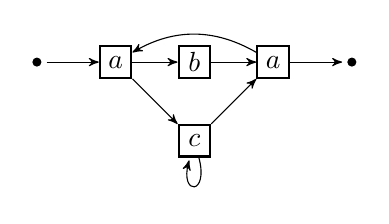
\begin{tikzpicture}[node distance=10mm,on grid,>=stealth',auto, sloped,state/.style={rectangle,draw=black,thick,inner sep=0pt,minimum size=4mm}]

	\node			(start)				{};
	\node[state]	(a1) [right=of start]{$a$};
	\node[state]	(b)[right=of a1]	{$b$};
	\node[state]	(c)[below=of b]	{$c$};
	\node[state]	(a2)[right=of b]	{$a$};
	\node 			(end)[right=of a2]	   	{};

	\draw[fill=black] (start) circle (0.5mm);
	\draw[fill=black] (end) circle (0.5mm);

	\draw[->]  (start) -- (a1);
	\draw[->]  (a1) -- (b);
	\draw[->]  (a1) -- (c);
	\draw[->]  (b) -- (a2);
	\draw[->]  (c) -- (a2);
	\draw[->]  (c) edge [loop below] (c);	
	\draw[->]  (a2) edge [bend right] (a1);
	\draw[->]  (a2) -- (end);
	\end{tikzpicture}
\end{center}
Every word in $L(\alpha)$ begins with an $a$, and this $a$ is always generated by the first occurrence of that letter in $\alpha$. Likewise, every word ends on $a$, and the final $a$ has to be generated by the second occurrence of $a$. The letters $b$ and $c$ always immediately follow an $a$ that was generated by the first occurrence of $a$, and are followed by an $a$ that was generated by the second occurrence. Due to the $\rxp$ after $c$, that letter loops to itself, and due to the outer $\rxp$, the second $a$ has an edge to the first one.
\end{example}

A full conversion algorithm is given with Algorithm~\ref{algo:OADRE} in Section~\ref{sec:OADRE}.

\paragraph{Deterministic Regular Expressions} We call a regular expression \emph{deterministic} if its canonical OA is deterministic. For example, the expressions $\alpha$ in Example~\ref{ex:oa} and the expression $a(ba)\rxp$ are deterministic, while the expression $(ab)\rxp a$ is not. This is easily seen by its canonical OA:
\begin{center}
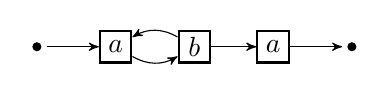
\begin{tikzpicture}[node distance=10mm,on grid,>=stealth',auto, sloped,state/.style={rectangle,draw=black,thick,inner sep=0pt,minimum size=4mm}]
	\node			(start)				{};
	\node[state]	(a1) [right=of start]{$a$};
	\node[state]	(b)[right=of a1]	{$b$};
	\node[state]	(a2)[right=of b]	{$a$};
	\node 			(end)[right=of a2]	   	{};

	\draw[fill=black] (start) circle (0.5mm);
	\draw[fill=black] (end) circle (0.5mm);

	\draw[->]  (start) -- (a1);
	\draw[->]  (a1) edge [bend right] (b);
	\draw[->]  (b) edge [bend right] (a1);
	\draw[->]  (b) -- (a2);
	\draw[->]  (a2) -- (end);
	\end{tikzpicture}
\end{center}
As the state with the label $b$ has two successors with the label $b$, we can conclude non-determinism. 

\paragraph{Equivalence Checking:} While it is possible to decide equivalence of DFAs via automata minimization, a less involved approach appears to be more suited for this implementation. The algorithm by Hopcroft and Karp~\cite{hop:lin} (see also Norton~\cite{nor:alg}) allows to decide equivalence in a more straightforward manner. Note that this algorithm can also be used to check for both possible directions of inclusion. The equivalence algorithm that is used in this project (Algorithm~\ref{algo:mew}) can be found in Section~\ref{algo:mew}.
%%%%%%%%%%%%%%%%%%%%%%%%%%%%%%%%%
\subsection{Normal Forms}
%%%%%%%%%%%%%%%%%%%%%%%%%%%%%%%%%
\paragraph{n-ary Normal Form:} The nNf of a regular expression is obtained by contracting all concatenation or choice nodes with children of the same type; i.\,e., $((a\ror b)\ror c)$ becomes $(a \ror b \ror c)$.

\paragraph{Plus Normal Form:} A central part of our approach to DREs is the use of a normal form, called the \emph{plus normal form (PNF)}. The PNF of a regular expression $\alpha$ in nNF is defined as $\nnf(\pnfup{\nnf(\wpnf{\alpha})})$, where the functions $\pnfupfun$ and $\wpnffun$ are defined below. 

Intuitively, $\wpnffun$ performs two tasks: The obvious one is the removal of all $\rxo$ operators that are applied to subexpressions which already generate $\emptyword$; the second one is that every special subexpression that occurs inside a star expression is broken up. For example, if $\alpha\df (a\rxo \rxc b\rxo)\rxp$, then $\wpnf{\alpha}= (a\ror b)\rxs$.

The function $\pnfupfun$ tries to move the option operators above the choice operators, if this is possible in a straightforward manner. For example, if $\beta\df (a\rxo \ror b\rxo)$, then $\pnfup{\beta}=(a\ror b)\rxo$. On the other hand, if one of the subexpressions of a choice expression is special, the function merely removes the option operator from all other subexpressions; e.\,g., if $\gamma\df ( a\rxo \ror (b\rxo\rxc c\rxo))$, then $\pnfup{\gamma}=(a \ror (b\rxo\rxc c\rxo) )$.

As the name suggests, the plus normal form is based on the star normal form from Brüggemann-Klein and Wood~\cite{bru:one}, incorporating the extension to the operator $\rxo$ by Gruber and Gulan~\cite{gru:sim}. (With the additional application of $\pnfupfun$.) Note that the plus normal form of an expression $\alpha\rxp$ is not identical to the star normal form of $(\alpha \rxc \alpha\rxs)$. 

The function $\wpnffun$ is defined by
\begin{align*}
	\wpnf{a}&\df a \text{ for every letter $a\in \Sigma$,}\\
	\wpnf{\alpha\rxp}
		&\df \begin{cases}
			\wpnfh{\wpnf{\alpha}}\rxp\rxo & \text{ if $\emptyword\in L(\alpha)$,}\\
			\wpnfh{\wpnf{\alpha}}\rxp & \text{ if $\emptyword\notin L(\alpha)$,}
		\end{cases}\\
	\wpnf{\alpha\rxo}
		&\df \begin{cases}
			\wpnf{\alpha} & \text{ if $\emptyword\in L(\alpha)$,}\\
			\wpnf{\alpha}\rxo & \text{ if $\emptyword\notin L(\alpha)$,}
		\end{cases}\\
	\wpnf{(\alpha_1\rxc \ldots \rxc \alpha_n)}
		&\df (\wpnf{\alpha_1}\rxc \ldots \rxc \wpnf{\alpha_n}),\\
	\wpnf{(\alpha_1\ror \cdots \ror \alpha_n)}
		&\df (\wpnf{\alpha_1} \ror \ldots \ror \wpnf{\alpha_n}),
\end{align*}
where the auxiliary function $\wpnfhfun$ is defined by 
\begin{align*}
	\wpnfh{a}&\df a\text{ for every letter $a\in \Sigma$,}\\
	\wpnfh{\alpha\rxp}
		&\df \alpha,\\
	\wpnfh{\alpha\rxo}
		&\df \alpha,\\
	\wpnfh{(\alpha_1\rxc \ldots \rxc \alpha_n)}
		&\df \begin{cases}
			(\wpnfh{\alpha_1}\ror \ldots \ror \wpnfh{\alpha_n}) & \text{if $\emptyword\in L((\alpha_1\rxc \ldots \rxc \alpha_n))$},\\
			(\alpha_1\rxc \ldots \rxc \alpha_n) & \text{if $\emptyword\notin L((\alpha_1\rxc \ldots \rxc \alpha_n))$},\\
		\end{cases}\\
	\wpnfh{(\alpha_1\ror \cdots \ror \alpha_n)}
		&\df (\wpnfh{\alpha_1}\ror \ldots \ror \wpnfh{\alpha_n}).
\end{align*}
We define $\pnfupfun$ by
\begin{align*}
	\pnfup{a}&\df a \text{ for all $a\in \Sigma$},\\
	\pnfup{\alpha\rxp}
		&\df \pnfup{\alpha}\rxp,\\
	\pnfup{\alpha\rxo}
		&\df \pnfup{\alpha}\rxo,\\
	\pnfup{(\alpha_1\rxc \ldots \rxc \alpha_n)}
		&\df (\pnfup{\alpha_1}\rxc \ldots \rxc \pnfup{\alpha_n}),\\
	\pnfup{(\alpha_1\ror \cdots \ror \alpha_n)}
		&\df \begin{cases}
			(\pnfup{\alpha_1}\ror \cdots \ror \pnfup{\alpha_n}) & \text{if $\emptyword\notin L((\alpha_1\ror \cdots \ror \alpha_n))$},\\
			(\pnfuph{\alpha_1}\ror \cdots \ror \pnfuph{\alpha_n})\rxo & \text{if $\emptyword\in L((\alpha_1\ror \cdots \ror \alpha_n))$}\\
			& \text{ and no $\alpha_i$ is special},\\
			(\pnfuph{\alpha_1}\ror \cdots \ror \pnfuph{\alpha_n})& \text{if there is a special $\alpha_i$}.
		\end{cases}
\end{align*}
where a regular expression $\alpha_i$ is called \emph{special} if it is a nullable concatenation.
Finally, the auxiliary function $\pnfuphfun$ is defined by
\begin{align*}
	\pnfuph{a}&\df a \text{ for all $a\in \Sigma$},\\
	\pnfuph{\alpha\rxp}
		&\df \pnfup{\alpha}\rxp,\\
	\pnfuph{\alpha\rxo}
		&\df \pnfup{\alpha},\\
	\pnfuph{(\alpha_1\rxc \ldots \rxc \alpha_n)}
		&\df (\pnfup{\alpha_1}\rxc \ldots \rxc \pnfup{\alpha_n}),\\
	\pnfuph{(\alpha_1\ror \cdots \ror \alpha_n)}
		&\df \pnfup{(\alpha_1\ror \cdots \ror \alpha_n)}.
\end{align*}
%%%%%%%%%%%%%%%%%%%%%%%%%%%%%%%%%
\subsection{Complexity Measures}
%%%%%%%%%%%%%%%%%%%%%%%%%%%%%%%%%
The three complexity measures $\siz$, $\syn$, and $\aw$ on regular expressions are defined as in Table~\ref{tab:measures}.
\begin{table}[h]
	\begin{tabular}[H]{|l||c|c|c|}
	\hline
	& $\siz$ & $\syn$ & $\aw$ \\
	\hline
	\hline
	$a\in\Sigma$ & 1 & 1 & 1 \\ \hline
	$\alpha\rxp$ & $3+\siz(\alpha)$ & $1+\syn(\alpha)$ & $\aw(\alpha)$\\ \hline 
	$\alpha\rxo$ & $3+\siz(\alpha)$ & $1+\syn(\alpha)$ & $\aw(\alpha)$\\ \hline 
	$(\alpha_1\rxc \ldots \rxc \alpha_n)$& $2+(n-1)+\sum \siz(\alpha_i)$& $(n-1) + \sum \syn(\alpha_i)$ & $\sum \aw(\alpha_i)$ \\ \hline
	$(\alpha_1\ror \cdots \ror \alpha_n)$& $2+(n-1)+\sum \siz(\alpha_i)$& $(n-1) + \sum \syn(\alpha_i)$ & $\sum \aw(\alpha_i)$ \\ \hline
	\end{tabular}
	\caption{\label{tab:measures} The definitions of the three complexity measures.}
\end{table}
The three measures can be interpreted as follows.
\begin{itemize}
	\item $\siz$ denotes the \emph{size} of the expression, i.\,e.\ the total number of symbols (terminals, operators, and parentheses).
	\item $\syn$ denotes the number of nodes in the binary syntax tree of the expression (hence, for n-ary operators, children beyond the second are penalized)
	\item $\aw$ denotes the \emph{alphabetic width} of the expression (i.\,e., the number of terminal letters).
\end{itemize}
%%%%%%%%%%%%%%%%%%%%%%%%%%%%%%%%%
\section{Algorithms}\label{sec:algo}
%%%%%%%%%%%%%%%%%%%%%%%%%%%%%%%%%
%%%%%%%%%%%%%%%%%%%%%%%%%%%%%%%%%
\subsection{The Conversion Algorithm \OAFromIndexedDRE}\label{sec:OADRE}
%%%%%%%%%%%%%%%%%%%%%%%%%%%%%%%%%
\begin{algorithm2e}[H]
	\SetKwInOut{Input}{input}
	\SetKwInOut{Output}{output}
	\SetKw{KwNot}{not}
	\SetKwData{delt}{D}
	\SetKwData{aut}{A}
	\SetKwData{Fset}{first}\SetKwData{Lset}{last}\SetKwData{Eset}{follow}\SetKwData{nullvar}{nullable}
	\Input{An indexed DRE \delt}
	\Output{None (this is a constructor)}
	\uIf{\delt is an (indexed) terminal}{
	$\Fset\leftarrow\{\delt\}$; $\Lset\leftarrow\{\delt\}$; $\Eset\leftarrow\emptyset$; $\nullvar\leftarrow \text{false}$; \Return{}\;
	}
	\uElseIf{\delt is a unary operator}{
		denote the (only) child of \delt by $\delt_1$\;
		$\aut_1\leftarrow \OAFromIndexedDRE(\delt_1)$\;
		$\Fset\leftarrow\aut_1.\Fset$; $\Lset\leftarrow\aut_1.\Lset$; $\Eset\leftarrow\aut_1.\Eset$\; 
		\If{\delt is an option}{
			$\nullvar\leftarrow \text{true}$; \Return{}\;
		}
		\Else(\tcc*[h]{\delt is a plus}){
			\lForEach{$u$ in $\aut_1.\Fset$, $v$ in $\aut_1.\Lset$}{add $(u,v)$ to \Eset}
			$\nullvar\leftarrow \aut_1.\nullvar$; \Return{}\;
		}
	}
	\Else(\tcc*[h]{\delt is an n-ary operator}){
		denote the children of \delt by $\delt_1$ to $\delt_n$ (from left to right)\;
		\If{\delt is a choice}{
			\lFor{$i\leftarrow 1$ \KwTo $n$}{$\aut_i\leftarrow \OAFromIndexedDRE(\delt_i)$}
			$\Fset\leftarrow \bigcup_{j=1}^{n} \aut_j.\Fset$;
			$\Lset\leftarrow \bigcup_{j=1}^{n} \aut_j.\Lset$\;
			$\Eset\leftarrow \bigcup_{j=1}^{n} \aut_j.\Eset$\;
			$\nullvar\leftarrow\bigvee_{j=1}^{n} \aut_j.\nullvar;$ \Return{}\;
		}
		\Else(\tcc*[h]{\delt is a concatenation}){
			\lIf{$n=2$}{$\aut_R\leftarrow\OAFromIndexedDRE(\delt_2)$}
			\lElse(\tcc*[h]{n>2}){$\aut_R\leftarrow\OAFromIndexedDRE((\delt_2\rxc\ldots\delt_n))$}
			\lIf{\KwNot $\aut_1.\nullvar$}{$\Fset\leftarrow \aut_1.\Fset$}
			\lElse{$\Fset\leftarrow \aut_1.\Fset\cup \aut_R.\Fset$}
			\lIf{\KwNot $\aut_R.\nullvar$}{$\Lset\leftarrow \aut_R.\Lset$}
			\lElse{$\Lset\leftarrow \aut_1.\Lset\cup \aut_R.\Lset$}
			$\Eset\leftarrow \aut_1.\Eset\cup\aut_R.\Eset$\;
			\lForEach{$u$ in $\aut_1.\Lset$, $v$ in $\aut_R.\Fset$}{add $(u,v)$ to \Eset}
			$\nullvar\leftarrow (\aut_1.\nullvar)\wedge(\aut_R.\nullvar)$;
			\Return{}\;
		}
	}
	\caption{\OAFromIndexedDRE\label{algo:OADRE}}
\end{algorithm2e}
%%%%%%%%%%%%%%%%%%%%%%%%%%%%%%%%%
\subsection{The OA~Equivalence mod $\emptyword$ Algorithm \equivalentToMEW}\label{sec:mew}
%%%%%%%%%%%%%%%%%%%%%%%%%%%%%%%%%
\begin{algorithm2e}[H]
	\SetAlgoLined
	\SetKwData{A}{A}\SetKwData{VA}{VA}\SetKwData{B}{B}\SetKwData{VB}{VB}	
	\SetKwData{qA}{qA}\SetKwData{qB}{qB}\SetKwData{rA}{rA}\SetKwData{rB}{rB}
	\SetKwData{lastSet}{L}\SetKwData{Mset}{Mset}
	\SetKwData{nodes}{nodes}\SetKwData{srcs}{src}\SetKwData{errs}{err}
	\SetKwData{S}{S}\SetKwData{U}{U}
	\SetKwFunction{makeset}{makeSet}
	\SetKwFunction{union}{union}
	\SetKwFunction{findFun}{find}
	\SetKwFunction{push}{push}
	\SetKwFunction{pop}{pop}
	\SetKwFunction{transfun}{delta}
	\SetKwFunction{lastFun}{last}
	\SetKwInOut{Input}{input}
	\SetKwInOut{Output}{output}
	\SetKwInOut{Assert}{assert}
	\Input{Occurrence automata \A, \B}
	\Output{\emph{true} if $L(\A)\setminus\{\emptyword\}=L(\B)\setminus\{\emptyword\}$, \emph{false} otherwise}
	\Assert{\A.\nodes() and \B.\nodes are disjoint\footnote{This is something the implementation has to ensure; e.\,g.\ by renaming indices.On the other hand, it might be preferable to leave the indices of the OAs unchanged, and handle this during $\makeset$.}.}
	\BlankLine
	$\VA \leftarrow \A.\nodes \cup \{\A.\srcs,\A.\errs\}$\;
	$\VB \leftarrow \B.\nodes \cup \{\B.\srcs,\B.\errs\}$\;
	\emph{initialize stack \S}\;
	\emph{initialize union-find structure\footnote{Also called disjoint set data structure. See any introduction to algorithms, e.\,g., Cormen et al.~\cite{cor:int}, Chapter~21. For now, a simple implementation suffices (e.\,g., via linked lists), as long as it is refactor the code without changing anything outside of the union-find data structure.} \U}\;
	\ForEach{element $v$ of $\VA\cup\VB$}{$\U.\makeset($v$)$}
	$\U.\union(\A.\srcs,\B.\srcs)$\;
	$\S.\push((\A.\srcs,\B.\srcs))$\;
	\While{\S is not empty}{
		$(\qA,\qB)\leftarrow \S.\pop()$\;
		\ForEach{$a\in\Sigma$}{
			$r_A\leftarrow \U.\findFun(\A.\transfun(\qA,a))$\;
			$r_B\leftarrow \U.\findFun(\B.\transfun(\qB,a))$\;
			\If{$\rA\neq\rB$}{
				$\U.\union(\rA,\rB)$\;
				$\S.\push(\rA,\rB)$\footnote{Instead of \rA,\rB, choose representatives from the respective sets.}\;
			}
		}
	}
	$\lastSet\leftarrow \A.\lastFun\cup \B.\lastFun()$\;
	\ForEach{set \Mset in \U}{
		\If{there exist elements $u,v$ in \Mset such that $u\in\lastFun$ and $v\notin\lastFun$}{
			\Return{\emph{false}}
		}
	}
	\Return{\emph{true}}
	\caption{\equivalentToMEW\label{algo:mew}} 
\end{algorithm2e}
% %%%%%%%%%%%%%%%%%%%%%%%%%%%%%%%%%
% \subsection{Algorithm for factoring out common suffixes}\label{sec:factor}
% %%%%%%%%%%%%%%%%%%%%%%%%%%%%%%%%%
% % %Procedure findCommonSuffix
% % \begin{procedure}[H]
% % 	\SetKwInOut{Input}{input}\SetKwInOut{Output}{output}\SetKwInOut{Assert}{assert}
% % 	\SetKwData{delt}{D}
% % 	\Input{}
% % 	
% % 	\caption{findCommonSuffix}
% % \end{procedure}
% 
% \begin{algorithm2e}[H]
% 	\SetAlgoLined
% 	\SetKwInOut{Input}{input}\SetKwInOut{Output}{output}\SetKwInOut{Assert}{assert}
% 	\SetKwData{delt}{D}
% 	\SetKwData{nh}{nothing_happened}
% 	
% 	
% 	\Input{A DRE \delt of type choice}
% 	\Output{A DRE that is equivalent to \delt and has no children with a common suffix}
% 	\BlankLine
% 	$\nh\leftarrow\text{true}$
% 	
% 	
% 	
% 	\caption{factorOut\label{algo:factor}}
% \end{algorithm2e}
%%%%%%%%%%%%%%%%%%%%%%%%%%%%%%%%%
\section{Specification}\label{sec:spec}
%%%%%%%%%%%%%%%%%%%%%%%%%%%%%%%%%
%%%%%%%%%%%%%%%%%%%%%%%%%%%%%%%%%
\subsection{Module}\label{sec:des:mod}
%%%%%%%%%%%%%%%%%%%%%%%%%%%%%%%%%
\begin{itemize}
	\item\texttt{DREfromString(str)} takes a string $s$, parses it into a DRE (exception if $s$ is not a representation of a DRE, in particular if expression is not deterministic). Some details:
	\begin{itemize}
		\item Do not assume that one letter in the string $s$ directly corresponds to one letter in $\Sigma$. A letter could be named \texttt{a1}, or \texttt{123}, or \texttt{alphaAlpha} (etc.). For now, assume that letters are defined by ``standard'' alphanumerical characters (i.\,e., \texttt{a-zA-Z0-9} -- case sensitive) and underscore (\texttt{\_}). If possible, try to avoid making extensions needlessly hard; but do not consider this a major design goal.
		\item For now, the concatenation operator can be represented with a comma. Consider that we might also decide to allow the use of whitespace as concatenation operator. Also, consider that whitespace might be allowed between parentheses or around operators. In other words, there might be a point where we want to consider the following three expressions equivalent. \begin{enumerate}
			\item \texttt{((a,b,a1)|b)}
			\item \texttt{((a b a1)|b)}
			\item \texttt{( (a b a1) | b)}
		\end{enumerate} 
		\item Optional: Allow use superfluous parentheses, e.\,g.\ $(((a)))$ instead of $a$
		\item Optional: Allow omission of parentheses (if unambiguity is preserved, or unambiguity modulo nNF). Can also be implemented for some operators only (e.\,g., allow $a?$ instead of $(a)?$).
		\item Optional: Allow use of \texttt{*} as shorthand. 
	\end{itemize}
%		\item\texttt{compareDREs(DRE, DRE)}  takes DREs $\alpha$ and $\beta$ and decides which of the four possible cases $L(\alpha)=L(\beta)$, $L(\alpha)\subset L(\beta)$, $L(\alpha)\supset L(\beta)$, or $L(\alpha)\incomp L(\beta)$ holds. (The symbol $\incomp$ denotes incomparability of sets.)  It is probably reasonable to use the appropriate automata for OAs.
\item\texttt{equivalentTo(OccurrenceAutomaton A, OccurrenceAutomaton B)} Returns \emph{true} if $A$ and $B$ are equivalent (i.\,e., $L(A)=L(B)$). Implement by returning \texttt{equivalentToMEW(A,B) and (A.nullable()==B.nullable())}.
\item\texttt{equivalentToMEW(OccurrenceAutomaton A, OccurrenceAutomaton B)} Returns \emph{true} if $A$ and $B$ are equivalent, modulo the empty word (i.\,e., $L(A)\setminus\{\emptyword\}=L(B)\setminus\{\emptyword\}$). See Algorithm~\ref{algo:mew} in Section~\ref{sec:mew}.

\end{itemize}
%%%%%%%%%%%%%%%%%%%%%%%%%%%%%%%%%
\subsection{\texttt{DRE}}\label{sec:des:dre}
%%%%%%%%%%%%%%%%%%%%%%%%%%%%%%%%%
\begin{itemize}
	\item\texttt{isDeterministic()} Returns whether the expression is deterministic. I suggest converting the expression into an \texttt{OccurrenceAutomaton} and calling the respective method.
	\item\texttt{isInNNF()} Returns whether the expression is in nNF.
	\item\texttt{toNNF()} Transforms the DRE into nNF.
	\item\texttt{isInPNF()} Returns whether the expression is in PNF.
	\item\texttt{toPNF()} Transforms the DRE into PNF.
	\item\texttt{terminals()} Returns the set (a list?) of the terminals that occur in the DRE (i.\,e., $\term(\alpha)$).
	\item\texttt{terminalOccurrences()} Returns a dictionary that maps every terminal in the DRE to its number of occurrences in the DRE.
	\item\texttt{first()} Returns the set (a list?) of the first letters of words in the language of the DRE.
	\item\texttt{getParent()} Returns reference to the DRE's parent.
	\item\texttt{leftSibling()} Returns reference to immediate left sibling of the DRE.
	\item\texttt{rightSibling()} Returns reference to immediate right sibling of the DRE.
	\item\texttt{getNextL2RBF()} Returns reference to next node in left-to-right breadth first search order.
	\item\texttt{size()} Returns the $\siz$ of the DRE.
	\item\texttt{rpn()} Returns the $\syn$ of the DRE.
	\item\texttt{awidth()} Returns the $\aw$ of the DRE.
	\item\texttt{toString()} Returns a string representation of the DRE. (Must be compatible with \texttt{DREfromString}, cf.\ Section~\ref{sec:des:mod}). Should be able to have an optional argument that states that combinations of $\rxp$ and $\rxo$ are printed as $\rxs$.
	\item\texttt{toDOTString()} Returns a tree representation of the DRE in the DOT format that is used by GraphViz (\url{http://www.graphviz.org/}). Use \texttt{ordering=out} to preserve the order. Consider using subgraphs, to further enforce this.
	\item \emph{Really, really optional:} \texttt{toTikZString()} Returns a tree representation of the DRE as a TikZ tree (\url{http://sourceforge.net/projects/pgf/}).
\end{itemize}
%%%%%%%%%%%%%%%%%%%%%%%%%%%%%%%%%
\subsection{\texttt{Nary}}\label{sec:des:nary}
%%%%%%%%%%%%%%%%%%%%%%%%%%%%%%%%%
\begin{itemize}
	\item\texttt{arity()} Returns the arity of the DRE node (i.\,e., the number of children).
\end{itemize}


%%%%%%%%%%%%%%%%%%%%%%%%%%%%%%%%%
\subsection{\texttt{IndexedDRE}}\label{sec:des:idre}
%%%%%%%%%%%%%%%%%%%%%%%%%%%%%%%%%
Extends \texttt{DRE} by adding indices to the terminal nodes. Indices are integers, and every index occurs only once (i.\,e., is characteristic for that terminal). Ideally, the indices start with 1 at the leftmost terminal symbol of the expression, and ascend accordingly. The rightmost index should be the alphabetic width of the expression. If this is too difficult, any other characteristic indexing function is fine, too.
\paragraph{Functions}
\begin{itemize}
	\item constructor, takes a (D)RE and adds indices
\end{itemize}

%%%%%%%%%%%%%%%%%%%%%%%%%%%%%%%%%
\subsection{\texttt{OccurrenceAutomaton}}\label{sec:des:oa}
%%%%%%%%%%%%%%%%%%%%%%%%%%%%%%%%%
\paragraph{Attributes}
\begin{itemize}
	\item\texttt{first} set of entry nodes (successors of $\src$)
	\item\texttt{last} set of exit nodes (predecessors of $\snk$)
	\item\texttt{follow} Set of edges (i.\,e., tuples of nodes). Might be empty (e.\,g., if the automaton accepts only a single letter). I suggest using a dictionary that maps nodes to sets of successors. 
	\item\texttt{nullable} True iff.\ the automaton accepts the empty word
	\item\texttt{src} constant that symbolizes the $\src$ node of the automaton
	\item\texttt{err} constant that symbolizes the failure node of the automaton	
\end{itemize}
Note that set set of vertices is not modeled explicitly. Furthermore, note that $\src$ and $\snk$ are not modeled as vertices, but via first, last, and nullable. In order to simplify the implementation, each nodes is modeled as a tuple of the label and some index.
\paragraph{Functions}
\begin{itemize}
	\item constructor, takes an indexed (D)RE (see Algorithm~\ref{algo:OADRE}, Section~\ref{sec:OADRE})
	\item\texttt{nodes()} Returns the set of all nodes (union of \texttt{first}, \texttt{last}, and first elements of elements of \texttt{follow}). 
	\item\texttt{labels()} Returns a set of all labels of nodes of the automaton (i.\,e., the terminals that occur in the OA).
	\item\texttt{isDeterministic()} Returns \emph{true} if the automaton is deterministic. (It is not deterministic if follow contains elements $(u,v_1)$ and $(u,v_2)$ such that $v_1$ and $v_2$ contain the same label.)
	\item\texttt{delta(node,terminal)}: When called with a node $u$ and a terminal $a$, computes the set of nodes $v$ such that $\lab(v)=a$, and $(u,v)\in\mathtt{follow}$. If it is easier, assume that the automaton is deterministic. If the set is empty, return the node \texttt{err}. Also, for every terminal \texttt{a}, define \texttt{delta(err,a)=err}.
%	\item\texttt{isComplete()} Returns \emph{true} if the automaton is complete.
%	\item\texttt{makeComplete()} Ensures that the automaton is complete: If there exists a node $u\in\mathtt{nodes()}$ and a terminal $a$ such that no successor if $u$ is labeled with $a$, introduce a new 
	\item\texttt{toDOTString()} Returns a tree representation of the automaton as an OA in the DOT format that is used by GraphViz  (\url{http://www.graphviz.org/}). Every state contains the terminal and an index, the edges are the edges from follow. Add a dot for $\src$ and $\snk$ and respective edges to elements of first or from elements of last.
	\item\texttt{toDOTStringDFA()} Returns a tree representation of the automaton as an DFA in the DOT format that is used by GraphViz. Every state contains the index as state name; terminals are written to the edges. Add an initial state which is connected to the states that correspond to elements of first, and make all states that correspond to elements of last accepting states.
\end{itemize}
%%%%%%%%%%%%%%%%%%%%%%%%%%%%%%%%%
\newpage
\section{Examples}\label{sec:exam}
%%%%%%%%%%%%%%%%%%%%%%%%%%%%%%%%%
%%%%%%%%%%%%%%%%%%%%%%%%%%%%%%%%%
\subsection{Plus Normal Form (Example~\ref{ex:pnf1})}
%%%%%%%%%%%%%%%%%%%%%%%%%%%%%%%%%
\begin{example}\label{ex:pnf1}
	Consider the deterministic regular expression 
	\[\alpha_1\df 
	((
		\mathtt{a}\rxo
	 		\ror 
		\mathtt{b}\rxo
	)\rxo
	\ror 
	(
		\mathtt{c}\rxo
	 		\ror 
		\mathtt{d}\rxo
	)\rxo)\rxo
	\]
	This expression is in nNF, and its parse tree is depicted in Figure~\ref{fig:parse-alpha}. Applying $\wpnffun$ to $\alpha_1$ leads to the DRE 
	\[
	\wpnf{\alpha_1}= ((\mathtt{a}\rxo \ror \mathtt{b}\rxo) \ror (\mathtt{c}\rxo \ror \mathtt{d}\rxo) )
	\]
	 which is depicted in Figure~\ref{fig:wpnf-alpha}. Note that $\wpnf{\alpha_1}$ is not in nNF; by converting it into nNF, we obtain the DRE 
	\[
	\nnf(\wpnf{\alpha_1})= (\mathtt{a}\rxo \ror \mathtt{b}\rxo \ror \mathtt{c}\rxo \ror \mathtt{d}\rxo),
	\]
	which is depicted in Figure~\ref{fig:nnf-wpnf-alpha}. Finally, the PNF of $\alpha_1$ is obtained by replacing the four occurrences of $\rxo$ with a single $\rxo$ operator over the $\ror$ (the $\rxo$ is moved by to the top). Formally, we apply the function, $\pnfupfun$ to create the PNF
	\[
	\pnfup{\nnf(\wpnf{\alpha_1})} = (\mathtt{a}\ror\mathtt{b}\ror\mathtt{c}\ror\mathtt{d})\rxo.
	\]
	The parse tree of this expression can be found in Figure~\ref{fig:pnf-alpha}.
	\begin{figure}
	\begin{center}
		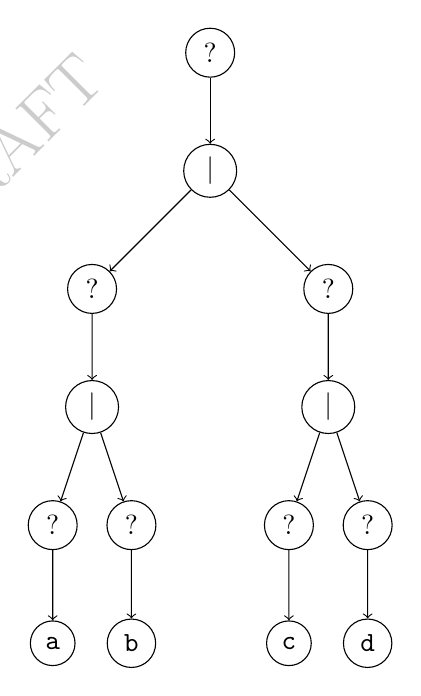
\begin{tikzpicture}[->,level 2/.style={sibling distance=30mm},level 3/.style={sibling distance=10mm}]
		\node[circle,draw] {$\rxo$} 
			child{
				node[circle,draw] {$\ror$} 
				child{
					node[circle,draw] {$\rxo$}
					child{
						node[circle,draw] {$\ror$}
						child{
							node[circle,draw] {$\rxo$}
							child{
								node[circle,draw]{\texttt{a}}
							}
						}
						child{
							node[circle,draw] {$\rxo$}
							child{
								node[circle,draw]{\texttt{b}}
							}
						}
					}
				}
				child{
					node[circle,draw] {$\rxo$}
					child{
						node[circle,draw] {$\ror$}
						child{
							node[circle,draw] {$\rxo$}
							child{
								node[circle,draw]{\texttt{c}}
							}
						}
						child{
							node[circle,draw] {$\rxo$}
							child{
								node[circle,draw]{\texttt{d}}
							}
						}
					}
				}
			}; 
		\end{tikzpicture}
	\end{center}
	\caption{\label{fig:parse-alpha}From Example~\ref{ex:pnf1}: The parse tree of the expression $\alpha_1=((\mathtt{a}\rxo\ror \mathtt{b}\rxo)\rxo\ror (\mathtt{c}\rxo\ror \mathtt{d}\rxo)\rxo)\rxo$.}
	\end{figure}
	\begin{figure}
		\begin{center}
			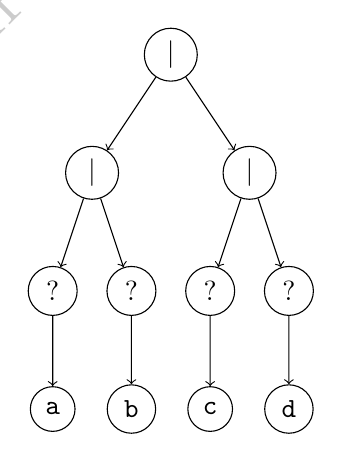
\begin{tikzpicture}[->,level 1/.style={sibling distance=20mm},level 2/.style={sibling distance=10mm}]
			\node[circle,draw] {$\ror$} 
				child{
					node[circle,draw] {$\ror$} 
					child{
						node[circle,draw] {$\rxo$}
						child{
							node[circle,draw] {\texttt{a}}
						}
					}
					child{
						node[circle,draw] {$\rxo$}
						child{
							node[circle,draw] {\texttt{b}}
						}
					}
				}
				child{
					node[circle,draw] {$\ror$} 
					child{
						node[circle,draw] {$\rxo$}
						child{
							node[circle,draw] {\texttt{c}}
						}
					}
					child{
						node[circle,draw] {$\rxo$}
						child{
							node[circle,draw] {\texttt{d}}
						}
					}
				};
			\end{tikzpicture}
		\end{center}
		\caption{\label{fig:wpnf-alpha}From Example~\ref{ex:pnf1}: The parse tree of the expression $\wpnf{\alpha_1}$.}
	\end{figure}
	\begin{figure}
		\begin{center}
			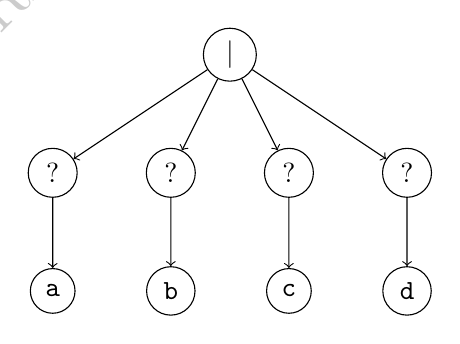
\begin{tikzpicture}[->]
			\node[circle,draw] {$\ror$} 
					child{
						node[circle,draw] {$\rxo$}
						child{
							node[circle,draw] {\texttt{a}}
						}
					}
					child{
						node[circle,draw] {$\rxo$}
						child{
							node[circle,draw] {\texttt{b}}
						}
					}
					child{
						node[circle,draw] {$\rxo$}
						child{
							node[circle,draw] {\texttt{c}}
						}
					}
					child{
						node[circle,draw] {$\rxo$}
						child{
							node[circle,draw] {\texttt{d}}
						}
					}
			;
			\end{tikzpicture}
		\end{center}
		\caption{\label{fig:nnf-wpnf-alpha}From Example~\ref{ex:pnf1}: The parse tree of the expression $\nnf(\wpnf{\alpha_1})$.}
	\end{figure}
	\begin{figure}
		\begin{center}
			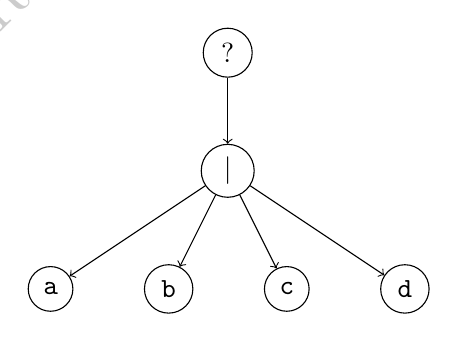
\begin{tikzpicture}[->]
			\node[circle,draw] {$\rxo$} 
					child{
						node[circle,draw] {$\ror$}
						child{
							node[circle,draw] {\texttt{a}}
						}
						child{
							node[circle,draw] {\texttt{b}}
						}
						child{
							node[circle,draw] {\texttt{c}}
						}
						child{
							node[circle,draw] {\texttt{d}}
						}
					}
			;
			\end{tikzpicture}
		\end{center}
		\caption{\label{fig:pnf-alpha}From Example~\ref{ex:pnf1}: The parse tree of the expression $\pnfup{\nnf(\wpnf{\alpha_1})}$, which is the PNF of $\alpha_1$.}
	\end{figure}
\end{example}
%%%%%%%%%%%
\subsection{Plus Normal Form (Example~\ref{ex:pnf2})}
\begin{example}\label{ex:pnf2}
	The PNF of the DRE
	\[ 
	\left(   
	\mathtt{a}\rxo
	\rxc
	\mathtt{b}\rxo
	\right)\rxp
	\]
	is 
	\[
	\left(\mathtt{a} \ror \mathtt{b}\right)\rxp\rxo
	\]
\end{example}
%%%%%%%%%%%
\subsection{Plus Normal Form (Example~\ref{ex:pnf3})}
\begin{example}\label{ex:pnf3}
	The PNF of the DRE
	\[
	\left( a\rxo \ror \left( b\rxo \rxc c\rxo \right)\right)\rxo 
	\]
	is 
	\[ \left(a \ror \left( b\rxo \rxc c\rxo  \right) \right)
	\]
\end{example}
%%%%%%%%%%%%%%%%%%%%%%%%%%%%%%%%%
\newpage
\section{Class Diagram}\label{sec:diag}
%%%%%%%%%%%%%%%%%%%%%%%%%%%%%%%%%
\begin{center}
\begin{tikzpicture}

\umlclass[type=abstract,x=2,y=0]{DRE}{}{}

\umlclass[x=0.8,y=-3]{Terminal}{}{}
\umlclass[type=abstract,x=4,y=-3]{Operator}{}{}
\umlclass[type=abstract,x=2,y=-7]{Unary}{}{}
\umlclass[type=abstract,x=6,y=-7]{Nary}{}{}

\umlclass[x=0.5,y=-10]{Optional}{}{}
\umlclass[x=3,y=-10]{Plus}{}{}
\umlclass[x=6,y=-10]{Concatenation}{}{}
\umlclass[x=9,y=-10]{Choice}{}{}

\umlinherit[geometry=|-|,anchor2=-110]{Terminal}{DRE}
\umlinherit[geometry=|-|,anchor2=-70]{Operator}{DRE}

\umlinherit[geometry=-|]{Unary}{Operator}
\umlinherit[geometry=-|]{Nary}{Operator}

%\umlaggreg[geometry=|-|,arm1=85mm,mult1=2..*,mult2=1]{Nary}{DRE}
\umlaggreg[geometry=|-,anchor2=10,mult2=2..*,mult1=1]{Nary}{DRE}
\umlaggreg[geometry=--,mult1=1,mult2=1]{Unary}{DRE}

\umlinherit[geometry=|-|]{Optional}{Unary}
\umlinherit[geometry=|-|]{Plus}{Unary}

\umlinherit[geometry=|-|]{Concatenation}{Nary}
\umlinherit[geometry=|-|]{Choice}{Nary}

%\umluniassoc[recursive=170|100|2cm,arg=parent]{DRE}{DRE}

\end{tikzpicture}
\end{center}
%%%%%%%%%%%%%%%%%%%%%%%%%%%%%%%%%
% REFERENCES
%%%%%%%%%%%%%%%%%%%%%%%%%%%%%%%%%
\newpage
\addcontentsline{toc}{section}{References}
\bibliographystyle{plain}
\bibliography{modod}
%%%%%%%%%%%%%%%%%%%%%%%%%%%%%%%%%%%%%%%%%%%%%%%
% TABLE OF CONTENTS
%%%%%%%%%%%%%%%%%%%%%%%%%%%%%%%%%%%%%%%%%%%%%%%
\newpage
\addcontentsline{toc}{section}{Contents}
\tableofcontents
\end{document}
